\chapter{Hybrid Context-Sensitivity}\label{chapter:hybrid}
%Hybrid Context-Sensitivity for Points-To Analysis

\epigraph{If you wanted to know about the Hybrid, why didn’t you just ask me?}{\textit{Doctor Who}}
%\epigraph{If your data fits in main memory, you're doing it wrong}{\textit{Anonymous}}

\emph{Points-to analysis} is a static program analysis that consists
of computing all objects (typically identified by allocation site)
that a program variable may point to. The area of points-to analysis
(and its close relative, \emph{alias analysis}) has been the focus of
intense research and is among the most standardized and
well-understood of inter-procedural analyses. The emphasis of
points-to analysis algorithms is on combining fairly precise modeling
of pointer behavior with scalability. The challenge is to pick
judicious approximations that will allow satisfactory precision at a
reasonable cost. Furthermore, although increasing precision often
leads to higher asymptotic complexity, this worst-case behavior is
rarely encountered in actual practice. Instead, techniques that are
effective at maintaining good precision often also exhibit better
average-case performance, since smaller points-to sets lead to less
work.

One of the major tools for exploiting sweet spots in the
precision/performance tradeoff has been \emph{context-sensitivity}.
Context-sensitivity consists of qualifying local variables and objects
with context information: the analysis unifies executions that map to
the same context value, while separating executions that map to
different contexts. This approach tries to counter the loss of
precision that naturally results in any static analysis from
conflating information from different dynamic program paths. Two main
kinds of context-sensitivity have been explored in the literature:
\emph{call-site-sensitivity}
\cite{Sharir:Interprocedural,thesis:Shivers} and
%Shivers:1988:CFA}
\emph{object-sensitivity}
\cite{issta:2002:Milanova,article:2005:Milanova,popl:2011:Smaragdakis}.

A call-site-sensitive/$k$CFA analysis uses method call-sites (i.e.,
labels of instructions that may call the method) as context elements.
That is, the analysis separates information on local variables (e.g.,
method arguments) per call-stack (i.e., sequence of $k$ call-sites) of
method invocations that led to the current method call. Similarly, the
analysis separates information on heap objects per call-stack of
method invocations that led to the object's allocation. For instance,
in the code example below, a 1-call-site-sensitive analysis (unlike a
\emph{context-insensitive} analysis) will distinguish the two
call-sites of method \code{foo} on lines 7 and 9. This means that the
analysis will treat \code{foo} separately for two cases: that of its
formal argument, \code{o}, pointing to anything \code{obj1} may point to, and
that of \code{o} pointing to anything \code{obj2} may point to.

\begin{figure}[h]
\begin{javacode}
class C {
 void foo(Object o) { ... }
}

class Client {
 void bar(C c1, C c2) { ...
   c1.foo(obj1);
   ...
   c2.foo(obj2);
 }
} 
\end{javacode}
\caption{Code snippet to illustrate context-sensitive analyses.}
\end{figure}

In contrast, object-sensitivity uses object allocation sites (i.e.,
labels of instructions containing a \code{new} statement) as context
elements. (Hence, a better name for ``object-sensitivity'' might have
been ``allocation-site sensitivity''.) That is, when a method is
called on an object, the analysis separates the inferred facts
depending on the allocation site of the receiver object (i.e., the
object on which the method is called), as well as other allocation
sites used as context. Thus, in the above example, a
1-object-sensitive analysis will analyze \code{foo} separately depending
on the allocation sites of the objects that \code{c1} and \code{c2} may
point to. It is not apparent from this code fragment neither whether
\code{c1} and \code{c2} may point to different objects, nor to how many
objects: the allocation site of the receiver object may be remote and
unrelated to the method call itself. Similarly, it is not possible to
compare the precision of an object-sensitive and a call-site-sensitive
analysis in principle. In this example, it is not even clear whether
the object sensitive analysis will examine all calls to \code{foo} as
one case, as two, or as many more, since this depends on the
allocation sites of all objects \emph{that the analysis itself computes to
flow into \code{c1} and \code{c2}}.

The question behind our work is whether the two kinds of contexts can
be fruitfully combined, since they are quite dissimilar. In order to
address this question, we map the design space of \emph{hybrid
  call-site- and object-sensitive} analyses and describe the
combinations that arise. Naive hybrids, such as always maintaining as
context \emph{both} a call-site and an allocation site, do not pay
off, due to extremely high cost. For instance, keeping one call-site
and one allocation site as context yields a very expensive analysis,
on average 3.9x slower than a simple 1-object-sensitive analysis.

%although it improves precision (yet not nearly as much as a
%2-object-sensitive analysis).

However, we find that more sophisticated hybrids are highly
beneficial. Specifically, we show that we can switch
per-language-feature between a combined context and an object-only
context. For instance, contexts for static method calls are computed
differently from contexts for dynamic method calls. This approach
yields analyses with both low cost and high precision.  Furthermore,
adapting contexts per program feature defines a complex design space
and allows even further optimization. Design choices arise, such as,
how should the context adapt when a dynamic method call, or an object
allocation are made inside a static method?

The end result is analyses that closely track the precision of
combined call-site-and-object-sensitivity while incurring none of the
cost. In fact, the cost of the resulting analysis is usually less
(and occasionally much less) than that of just an object-sensitive
analysis, due to increased precision. This effect is shown to apply
widely, to several variants of analyses. Accordingly, this outcome
establishes new sweet spots for the analyses most relevant for
practical applications: 1-object-sensitive, 2-object-sensitive with a
1-context-sensitive heap, and analogous type-sensitive
\cite{popl:2011:Smaragdakis} analyses. For all of them, a selective hybrid
context is typically both more precise and faster than the original
analysis. 

%The effect is very clear and surprising, even to ourselves:
%Although on the onset of our work we expected at best to see a small
%benefit over existing ``highly effective'' object-sensitive analyses,
%we observe for several benchmarks speedups of over 300\%, combined
%with higher precision. 

%Although in principle call-site- and object-sensitivity are
%incomparable, in practice the story is quite
%clear. Call-site-sensitivity has a long history, dating to at least
%the '80s. For a long time, call-site-sensitivity was considered
%synonymous with context-sensitivity as a whole. Object-sensitivity was
%introduced in 2002 \cite{issta:2002:Milanova} and within a
%decade it has become the overwhelming choice of context-sensitivity
%for object-oriented programs. Multiple studies
%\cite{NaikAikenWhaley2006,DBLP:conf/paste/LiangPH05,thesis:Lhotak,article:2008:tosem:Lhotak,oopsla:2009:Bravenboer}
%have found object-sensitive analyses to yield excellent precision/cost
%tradeoffs. Compared to call-site-sensitive/$k$CFA analyses, an
%object-sensitive analysis of the same context depth has always been
%advantageous, in terms of both speed and performance. 

%Given such past experimental results, it would seem that exploring
%combinations of call-site- and object-sensitivity is futile. There is
%no tradeoff to exploit. Even though call-site-sensitive analyses are
%occasionally faster to execute, this only comes at the expense of
%precision. To achieve the same precision target as an object-sensitive
%analysis, call-site-sensitive analyses have to suffer much higher
%cost.  Additionally, coarser approximations of object-sensitivity,
%such as \emph{type-sensitivity} \cite{popl:2011:Smaragdakis} have filled the
%performance gap and offered fast options for cases when a full
%object-sensitive analysis is too expensive.

%Our work shows that this conventional wisdom is false. 


In all, our paper makes the following contributions:

\begin{itemize}
\item We model the parameter space of context-sensitive points-to
  analysis in a way that allows both call-site- and
  object-sensitivity, as well as combinations and switching of context
  at key points (virtual calls vs. static calls). In this space, we
  map out choices that produce entirely different flavors of
  algorithms.

\item We introduce the idea of hybrid call-site- and
  object-sensitivity where the two kinds of context are freely mixed
  and the mix is adjusted in response to analyzing different program
  features. The goal is to achieve the precision of keeping
  \emph{both} kinds of context together, but at the same cost as
  keeping only one.

\item We implement our approach in the \doop{} framework
  by Bravenboer et al. \cite{oopsla:2009:Bravenboer} and apply it to a large
  variety of algorithms with varying context depth.

\item We show experimentally, over large Java benchmarks and the Java
  JDK, that hybrid context-sensitivity works remarkably well. 
%Our experiments establish that different programming language
% constructs are best analyzed with different kinds of context.
  The selective application of a combined context achieves the same
  effective precision as keeping both contexts at all times, at a
  fraction of the cost, and is typically faster even than keeping only
  an object context. For instance, in the practically important case
  of a 2-object-sensitive analysis with a context-sensitive heap, we
  get an average speedup of 1.53x \emph{and} a more precise
  analysis. Similarly, for the simple and popular 1-object-sensitive
  analysis, we get an average speedup of 1.12x combined with significant
  increase in precision.

%  This is one of the rare occasions when the combination of two ideas
%  supplants both: hybrid context-sensitivity outperforms both object-
%  and call-site-sensitivity in both precision and speed.
\end{itemize}

The rest of the paper introduces a model for points-to analysis
(Section~\ref{sec:model}) and shows how instantiating the model yields
several well-known analyses. In Section~\ref{sec:hybrid} we discuss the many
choices for combining object- and call-site-sensitivity, as well as
the most promising points in this design space. Our evaluation results
follow in Section~\ref{sec:evaluation}, before describing related work
(Section~\ref{sec:related}).

% \begin{comment}

% In this paper, we offer a unified formal framework that captures the
% object-sensitive analyses defined in the literature and allows a
% deeper understanding of their differences. Additionally, we implement
% an array of object-sensitive analyses and draw insights about how the
% choice of context relates to scalability and precision. We discover
% that the seemingly simple difference of how an analysis context is
% chosen results in large differences in precision and performance. We
% use the name \emph{full-object sensitivity} to refer to (a slight
% generalization of) the original statement of object-sensitivity by
% Milanova et al.
% % A ``full-object sensitive'' analysis uses the full abstract receiver
% %object (or as much of it as allowed by the analysis parameters) as
% %context for a called method.
% We argue that full-object sensitivity is an excellent choice in the
% design space, while the choice of context made in past actual
% implementations 
% %(mainly of the \textsc{Paddle} framework
% %\cite{thesis:Lhotak,1377494}) 
% is sub-optimal and results in substantial loss of
% precision. Concretely, a practical outcome of our work is to establish
% a 2-full-object-sensitive analysis with a 1-object-sensitive heap
% (shortened to ``2full+1H'') as an analysis that is often (though not
% always) feasible with current technology and impressively precise.
% %For a rough illustration,
% %a 2full+1H analysis improves over the precision of a
% %traditional-context 2obj+1H analysis by amounts comparable to those
% %observed when switching from a context-insensitive analysis to a
% %1obj+1H analysis (largely considered the current state-of-the-art
% %feasible and precise analysis).

% Perhaps even more importantly, our understanding of the impact of
% context on the effectiveness of an analysis leads to defining a new
% variant that combines scalability with good precision.  Namely, we
% introduce the idea of a \emph{type-sensitive} analysis, which is
% defined to be directly analogous to an object-sensitive analysis, yet
% approximates (some) context elements using types instead of full
% allocation sites. In contrast to past uses of types in points-to
% analysis (e.g.,
% \cite{Sundaresan:2000:PVM,Agesen:1995:CPA:646153.679533,Plevyak:1994:PCT:191080.191130}
% and see Ryder \cite{Ryder:2003:DPR} for several examples) we
% demonstrate that the types used as contexts should \emph{not} be the
% types of the corresponding objects. Instead, the precision of our
% type-sensitive analysis is due to replacing the allocation site of an
% object $o$ (which would be used as context in an object-sensitive
% analysis) with an upper-bound of the dynamic type of $o$'s allocator
% object.  The result is a substantial improvement that establishes a
% new sweet spot in the practical tradeoff of points-to analysis
% precision and performance.

% \end{comment}



\section{Modeling of Points-To Analysis}
\label{sec:model}

We begin with a concise modeling of the relevant points-to analyses
and their context choices.

\subsection{Background: Parameterizable Model}

We model a spectrum of flow-insensitive points-to analyses and joint
(online) call-graph construction as a parametric Datalog program.
Datalog rules are monotonic logical inferences that repeatedly apply
to infer more facts until fixpoint. Our rules do not use negation in a
recursive cycle, or other non-monotonic logic constructs, resulting in
a declarative specification: the order of evaluation of rules or
examination of clauses cannot affect the final result. The same
abstract model applies to a wealth of analyses. We use it to model a
context-insensitive Andersen-style \cite{thesis:Andersen}
analysis, as well as several context-sensitive analyses, both
call-site-sensitive and object-sensitive.

The input language is a representative simplified intermediate
language with a) a ``new'' instruction for allocating an object; b) a
``move'' instruction for copying between local variables; c) ``store''
and ``load'' instructions for writing to the heap (i.e., to object
fields); d) a ``virtual method call'' instruction that calls the
method of the appropriate signature that is defined in the dynamic
class of the receiver object; e) a ``static method call'' instruction
that calls a statically known target method. This language models well
the Java bytecode representation, but also other high-level
intermediate languages.  (It does not, however, model languages such
as C or C++ that can create pointers through an address-of
operator. The techniques used in that space are fairly
different---e.g., \cite{pldi:2007:Hardekopf,popl:2009:Hardekopf}---although our main
hybrid approach is likely to be applicable. Also, even though we
model regular object fields and static methods, we omit static fields.
Their treatment is a mere engineering complexity, as it does not
interact with context choice.) The specification of our points-to
analysis as well as the input language are in line with those in past
literature \cite{uss:2009:Guarnieri,sigsoft:2013:Madsen},
although we also integrate elements such as on-the-fly call-graph
construction, static calls, and field-sensitivity.

Specifying the analysis logically as Datalog rules has the advantage
that the specification is close to the actual implementation.  Datalog
has been the basis of several implementations of program analyses,
both low-level
\cite{repsdb,aplas:2005:Whaley,pods:2005:Lam,pldi:2004:Whaley,oopsla:2009:Bravenboer}
and high-level \cite{icse:2008:Eichberg,ecoop:2006:Hajiyev}. Indeed, the analysis we show
is a faithful model of the implementation in the \doop{}
framework~\cite{oopsla:2009:Bravenboer}, upon which our work builds. Our
specification of the analysis
(Figures~\ref{fig:input}-\ref{fig:baserules}) is an abstraction of the
actual implementation in the following ways:

\begin{itemize}
\item The implementation has many more rules. It covers the full
  complexity of Java, including rules for handling reflection, native
  methods, static fields, string constants, implicit initialization,
  threads, and a lot more. The \doop{}
  implementation\footnote{Available at
    http://doop.program-analysis.org/} currently contains over 600
  rules in the common core of all analyses, and several more rules
  specific to each analysis, as opposed to the 9 rules we examine
  here. (Note, however, that these few rules are the most crucial for
  points-to analysis. They also correspond fairly closely to the
  algorithms specified in other formalizations of points-to analyses
  in the literature~\cite{pldi:2010:Might,popl:2011:Smaragdakis}.)

\item The implementation also reflects considerations for efficient
  execution. The most important is that of defining indexes for the
  key relations of the evaluation. Furthermore, it designates some
  relations as functions, defines storage models for relations (e.g.,
  how many bits each variable uses), designates intermediate relations
  as ``materialized views'' or not, etc. No such considerations are
  reflected in our model.
\end{itemize}

%\vspace{-5mm}
\begin{figure}[tb!p]
%\begin{center}
\hspace{-1mm}
\begin{tabular}{l}
%\begin{tabular}{llll}
%$V$ is a set of variables & $H$ is a set of heap abstractions \\
%$M$ is a set of methods & $S$ is a set of method signatures (including name) \\
%$F$ is a set of fields & $I$ is a set of instructions (e.g., invocation sites)\\
%$T$ is a set of class types & $\mathbb{N}$ is the set of natural numbers \\
%$HC$ is a set of heap contexts & $C$ is a set of contexts \\
%\end{tabular}
\small $V$ is a set of program variables \\
\small $H$ is a set of heap abstractions (i.e., allocation sites) \\
\small $M$ is a set of method identifiers \\
\small $S$ is a set of method signatures (including name, type signature) \\
\small $F$ is a set of fields \\
\small $I$ is a set of instructions (mainly used for invocation sites)\\
\small $T$ is a set of class types \\
\small $\mathbb{N}$ is the set of natural numbers \\
\small $C$ is a set of contexts \\
\small $HC$ is a set of heap contexts \\
%\\
\cline{1-1}
%\begin{tabular}{ll}
%\pred{Alloc}{var : V, heap : H, inMeth : M}   &   \pred{FormalArg}{meth : M, i : $\mathbb{N}$, arg : V} \\ 
%\pred{Move}{to : V, from : V}               &   \pred{ActualArg}{invo : I, i : $\mathbb{N}$, arg : V} \\ 
%\pred{Load}{to : V, base : V, fld : F}      &   \pred{FormalReturn}{meth : M, ret : V} \\                
%\pred{Store}{base : V, fld : F, from : V}   &   \pred{ActualReturn}{invo : I, var : V} \\                
%\pred{VCall}{base : V, sig : S, invo : I, inMeth : M}   &   \pred{ThisVar}{meth : M, this : V} \\                    
%\pred{SCall}{meth : M, invo : I, inMeth : M}&   \pred{HeapType}{heap : H, type : T} \\
%                                            &   \pred{LookUp}{type : T, sig : S, meth : M} \\            
%\pred{InMethod}{instr : I, meth : M}        &   \pred{Subtype}{type : T, superT : T} \\
%\end{tabular}
\hspace{-3mm}
\begin{tabular}{l l}
\pred{Alloc}{var : V, heap : H, inMeth : M}  & \args{\# var = new ...} \\
\pred{Move}{to : V, from : V}                & \args{\# to = from} \\
\pred{Load}{to : V, base : V, fld : F}       & \args{\# to = base.fld}\\
\pred{Store}{base : V, fld : F, from : V}    & \args{\# base.fld = from} \\
\pred{VCall}{base : V, sig : S, invo : I, inMeth : M} & \args{\# base.sig(..)}   \\
\pred{SCall}{meth : M, invo : I, inMeth : M} & \args{\# Class.meth(..)}\\
\end{tabular}\\
\\
\pred{FormalArg}{meth : M, i : $\mathbb{N}$, arg : V} \\ 
\pred{ActualArg}{invo : I, i : $\mathbb{N}$, arg : V} \\ 
\pred{FormalReturn}{meth : M, ret : V} \\                
\pred{ActualReturn}{invo : I, var : V} \\                
\pred{ThisVar}{meth : M, this : V} \\                    
\pred{HeapType}{heap : H, type : T} \\
\pred{LookUp}{type : T, sig : S, meth : M} \\            
%\\
\cline{1-1}
\pred{VarPointsTo}{var : V, ctx : C, heap : H, hctx : HC} \\
\pred{CallGraph}{invo : I, callerCtx : C, meth : M, calleeCtx : C} \\
\pred{FldPointsTo}{baseH: H, baseHCtx: HC, fld: F, heap: H, hctx: HC} \\
\pred{InterProcAssign}{to : V, toCtx : C, from : V, fromCtx : C} \\
\pred{Reachable}{meth : M, ctx : C} \\
%\\
\cline{1-1}
\cons{Record}{heap : H, ctx : C}{newHCtx : HC} \\
\cons{Merge}{heap : H, hctx : HC, invo : I, ctx : C}{newCtx : C} \\
\cons{MergeStatic}{invo : I, ctx : C}{newCtx : C} \\
%\\
%\cline{1-1}
\end{tabular}
%\end{center}
\caption[]{Our domain, input relations (representing program instructions---with
the matching program pattern shown in a comment---and type
information), output relations, and constructors of contexts.}
\label{fig:input}
\end{figure}


\begin{figure}[tb!p]
%\begin{center}
\begin{tabular}{l}
%\cline{1-1}
\pred{InterProcAssign}{to, calleeCtx, from, callerCtx} $\leftarrow$ \\
\tab \pred{CallGraph}{invo, callerCtx, meth, calleeCtx}, \\
\tab \pred{FormalArg}{meth, i, to}, \pred{ActualArg}{invo, i, from}. \\
\\

\pred{InterProcAssign}{to, callerCtx, from, calleeCtx} $\leftarrow$ \\
\tab \pred{CallGraph}{invo, callerCtx, meth, calleeCtx}, \\
\tab \pred{FormalReturn}{meth, from}, \pred{ActualReturn}{invo, to}. \\
\\
\\
\cons{Record}{heap, ctx}{hctx}, \\
\pred{VarPointsTo}{var, ctx, heap, hctx} $\leftarrow$ \\
\tab \pred{Reachable}{meth, ctx}, \pred{Alloc}{var, heap, meth}. \\
\\

\pred{VarPointsTo}{to, ctx, heap, hctx} $\leftarrow$ \\
\tab \pred{Move}{to, from}, \pred{VarPointsTo}{from, ctx, heap, hctx}. \\
\\

\pred{VarPointsTo}{to, toCtx, heap, hctx} $\leftarrow$ \\
\tab \pred{InterProcAssign}{to, toCtx, from, fromCtx}, \\
\tab \pred{VarPointsTo}{from, fromCtx, heap, hctx}. \\
\\

\pred{VarPointsTo}{to, ctx, heap, hctx} $\leftarrow$ \\
\tab \pred{Load}{to, base, fld}, \pred{VarPointsTo}{base, ctx, baseH, baseHCtx}, \\
\tab \pred{FldPointsTo}{baseH, baseHCtx, fld, heap, hctx}. \\
\\

\pred{FldPointsTo}{baseH, baseHCtx, fld, heap, hctx} $\leftarrow$ \\
\tab \pred{Store}{base, fld, from}, \pred{VarPointsTo}{from, ctx, heap, hctx},\\
\tab \pred{VarPointsTo}{base, ctx, baseH, baseHCtx}. \\
\\
\\
\cons{Merge}{heap, hctx, invo, callerCtx}{calleeCtx}, \\
\pred{Reachable}{toMeth, calleeCtx}, \\
\pred{VarPointsTo}{this, calleeCtx, heap, hctx}, \\
\pred{CallGraph}{invo, callerCtx, toMeth, calleeCtx} $\leftarrow$ \\
\tab \pred{VCall}{base, sig, invo, inMeth}, \pred{Reachable}{inMeth, callerCtx}, \\
\tab \pred{VarPointsTo}{base, callerCtx, heap, hctx},\\
\tab \pred{HeapType}{heap, heapT}, \pred{Lookup}{heapT, sig, toMeth},\\
\tab \pred{ThisVar}{toMeth, this}. \\
\\

\cons{MergeStatic}{invo, callerCtx}{calleeCtx}, \\
\pred{Reachable}{toMeth, calleeCtx}, \\
\pred{CallGraph}{invo, callerCtx, toMeth, calleeCtx} $\leftarrow$ \\
\tab \pred{SCall}{toMeth, invo, inMeth}, \pred{Reachable}{inMeth, callerCtx}. \\
%\cline{1-1}
\end{tabular}
%\end{center}
\caption[]{Datalog rules for the points-to analysis and call-graph construction.}
\label{fig:baserules}
\end{figure}

Figure~\ref{fig:input} shows the domain of our analysis (i.e., the
different value sets that constitute the space of our computation),
its input relations, the intermediate and output relations, as well as
three constructor functions, responsible for producing new
contexts. Figure~\ref{fig:baserules} shows the points-to analysis and
call-graph computation.  The rule syntax is simple: the left arrow
symbol ($\leftarrow$) separates the inferred facts (i.e., the
\emph{head} of the rule) from the previously established facts (i.e.,
the \emph{body} of the rule). For instance, the first rule states
that, if we have computed a call-graph edge between invocation site
\args{invo} and method \args{meth} (under some contexts---see later),
then we infer an inter-procedural assignment to the $i$-th formal
argument of \args{meth} from the $i$-th actual argument at
\args{invo}, for every $i$.

We explain the contents of both figures in more detail below:

\begin{itemize}
\item The input relations correspond to the intermediate language for
  our analysis. They are logically grouped into relations that
  represent instructions and relations that represent name-and-type
  information. For instance, the \predname{Alloc} relation represents
  every instruction that allocates a new heap object, \args{heap}, and
  assigns it to local variable \args{var} inside method
  \args{inMeth}. (Note that every local variable is defined in a
  unique method, hence the \args{inMeth} argument is also implied by
  \args{var} but is included to simplify later rules.) There are similar
  input relations for all other instruction types (\predname{Move},
  \predname{Load}, \predname{Store}, \predname{VCall}, and
  \predname{SCall}). Similarly, there are relations that encode
  pertinent symbol table information.  Most of these are
  self-explanatory but some deserve explanation. \predname{LookUp}
  matches a method signature to the actual method definition inside a
  type. \predname{HeapType} matches an object to its type, i.e., is a
  function on its first argument. (Note that we are shortening the
  term ``heap object'' to just ``heap'' and represent heap objects as
  allocation sites throughout.) \predname{ActualReturn} is also a
  function on its first argument (a method invocation site) and
  returns the local variable at the call-site that receives the method
  call's return value.
  
\item There are five output or intermediate computed relations
  (\predname{VarPointsTo}, $\ldots$, \predname{Reachable}). Every
  occurrence of a method or local variable in computed relations is
  qualified with a context (i.e., an element of set \args{C}), while
  every occurrence of a heap object is qualified with a heap context
  (i.e., an element of \args{HC}). The main output relations are
  \predname{VarPointsTo} and \predname{CallGraph}, encoding our
  points-to and call-graph results. The \predname{VarPointsTo}
  relation links a variable (\args{var}) to a heap object
  (\args{heap}). Other intermediate relations (\predname{FldPointsTo},
  \predname{InterProcAssign}, \predname{Reachable}) correspond to
  standard concepts and are introduced for conciseness. For instance,
  \predname{InterProcAssign} (which encodes all parameter and return
  value passing) unifies much of the treatment of static and virtual
  method calls.

\item The base rules are not concerned with what kind of
  context-sensitivity is used. The same rules can be used for a
  context-insensitive analysis (by only ever creating a single context
  object and a single heap context object), for a call-site-sensitive
  analysis, or for an object-sensitive analysis, for any context
  depth. These aspects are completely hidden behind constructor
  functions \consname{Record}, \consname{Merge}, and
  \consname{MergeStatic}. The first two follow the usage and naming
  convention of Smaragdakis et al.~\cite{popl:2011:Smaragdakis}, while
  \consname{MergeStatic} is new and used to differentiate the
  treatment of static calls---this is a crucial element of our approach.

  \consname{Record} is the function that creates a new heap context.
  It is invoked whenever an object allocation site (input relation
  \predname{Alloc}) is analyzed. Thus, \consname{Record} is only used
  in the rule treating allocation instructions (3rd rule in
  Figure~\ref{fig:baserules}). \consname{Record} takes all available
  information at the allocation site of an object and combines it to
  produce a new heap context. The rule merely says that an allocation
  instruction in a reachable method leads us to infer a points-to
  fact between the allocated object and the variable it is directly
  assigned to.

  \consname{Merge} and \consname{MergeStatic} are used to create new
  calling contexts (or just ``contexts''). These contexts are used to
  qualify method calls, i.e., they are applied to all local variables
  in a program. The \consname{Merge} and \consname{MergeStatic}
  functions take all available information at the call-site of a
  method (virtual or static) and combine it to create a new context
  (if one for the same combination of parameters does not already
  exist). These functions are sufficient for modeling a very large
  variety of context-sensitive analyses, as we show in Sections
  \ref{sec:instances} and \ref{sec:hybrid}.

  Note that the use of constructors, such as \consname{Record},
  \consname{Merge}, and \consname{MergeStatic}, is not part of regular
  Datalog and can result in infinite structures (e.g., one can express
  unbounded call-site sensitivity) if care is not taken. All our later
  definitions statically guarantee to create contexts of a pre-set
  depth.

\item The rules of Figure~\ref{fig:baserules} show how each input
  instruction leads to the inference of facts for the five output or
  intermediate relations. The most complex rule is the second-to-last,
  which handles virtual method calls (input relation
  \predname{VCall}). The rule says that if a reachable method of the
  program has an instruction making a virtual method call over local
  variable \args{base} (this is an input fact), and the analysis so
  far has established that \args{base} can point to heap object
  \args{heap}, then the called method is looked up inside the type of
  \args{heap} and several further facts are inferred: that the looked
  up method is reachable, that it has an edge in the call-graph from
  the current invocation site, and that its \args{this} variable can
  point to \args{heap}. Additionally, the \consname{Merge} function is
  used to possibly create (or look up) the right context for the
  current invocation.



%To give a single example, however, a
%1-call-site-sensitive analysis with a context-sensitive heap has
%$C = HC = I$ (i.e., both the context and the heap context are a
%single instruction), \cons{Record}{heap, ctx}{ctx} and
%\cons{Merge}{heap, hctx, invo, callerCtx}{invo}. That is, when an
%object is allocated, its (heap) context is that of the allocating
%method, and when a method is called, its context is its call-site.}

%For instance, for a 1-call-site-sensitive analysis,
%\cons{Merge}{heap, hctx, invo, callerCtx}{invo}. For a
%1-object-sensitive analysis, \cons{Merge}{heap, hctx, invo,
%callerCtx}{heap}.

\end{itemize}


\subsection{Instantiating the Model: Standard Analyses}
\label{sec:instances}

By modifying the definitions of the \consname{Record},
\consname{Merge} and \consname{MergeStatic} functions as well as
domains \args{HC} and \args{C}, one can create endless variations of
points-to analyses. We next discuss the most interesting combinations
from past literature, before we introduce our own (in
Section~\ref{sec:hybrid}).  For every analysis name we also list a
common abbreviation, which we often use later.

\paragraph{Context-insensitive (insens).}
As already mentioned, our context-sensitive analysis framework can
yield a context-insensitive analysis by merely picking singleton
\args{C} and \args{HC} sets (i.e., \args{C} = \args{HC} =
\args{\{$\star$\}}, where $\star$ is merely a name for a distinguished
element) and constructor functions that return the single element of
the set:
\begin{quote}
\cons{Record}{heap,ctx}{$\star$}\\
\cons{Merge}{heap, hctx, invo, ctx}{$\star$} \\
\cons{MergeStatic}{invo, ctx}{$\star$}
\end{quote}

\noindent Note that the absence of contexts does not mean that the
identity of input elements is forgotten. Objects are still represented
by their allocation site (i.e., the exact program instruction that
allocated the object) and local variables are still distinguished
(e.g., by their declaration location in the input program). The
absence of context just means that there is no \emph{extra}
distinguishing information. This can also be seen in the rules of
Figure~\ref{fig:baserules}, where the \args{var} and \args{heap}
predicate arguments are present, separately from the context
arguments.

\paragraph{1-call-site-sensitive (1call).}
A 1-call-site-sensitive analysis has no heap context to qualify heap
abstractions (\args{HC} = \args{\{$\star$\}}) and uses the current
invocation site as a context (\args{C} = \args{I}). The following
definitions describe such an analysis.
\begin{quote}
\cons{Record}{heap, ctx}{$\star$} \\
\cons{Merge}{heap, hctx, invo, ctx}{invo} \\
\cons{MergeStatic}{invo, ctx}{invo}
\end{quote}
In words: the analysis stores no context when an object is created
(\consname{Record}) and keeps the invocation site as context in
both virtual and static calls.

\paragraph{1-call-site-sensitive with a context-sensitive
heap (1call+H).} The analysis is defined similarly to
1call.\footnote{The standard convention in the points-to analysis
literature is to name an analysis first according to the context of
methods, and, if a heap context exists, designate it in a suffix such
as \emph{context-sensitive heap} or \emph{heap cloning}.}  The heap
context as well as the main context consist of an invocation site
(\args{HC} = \args{C} = \args{I}).
\begin{quote}
\cons{Record}{heap, ctx}{ctx} \\
\cons{Merge}{heap, hctx, invo, ctx}{invo} \\
\cons{MergeStatic}{invo, ctx}{invo} 
\end{quote}
In words: the analysis uses the current method's context as a heap
context for objects allocated inside the method. The invocation site
of a method call is the context of the method for both virtual and
static calls.

\paragraph{1-object-sensitive (1obj).}
Object sensitivity uses allocation sites as context components. A
1-object-sensitive analysis has no heap context (\args{HC} =
\args{\{$\star$\}}) and uses the allocation site of the receiver
object as context (\args{C} = \args{H}). The following definitions
complete the description. 
\begin{quote}
\cons{Record}{heap, ctx}{$\star$} \\
\cons{Merge}{heap, hctx, invo, ctx}{heap} \\
\cons{MergeStatic}{invo, ctx}{ctx} 
\end{quote}
In words: the analysis stores no context for allocated objects. For
virtual method calls, the context is the allocation site of the
receiver object. For static method calls, the context for the called
method is that of the calling method.

The above definition offers a first glimpse of the possibilities that
we explore in this paper, and can serve as motivation. In static
calls, the context of the caller method is copied, i.e., the receiver
object of the caller method is used as the new context. Why not try
\cons{MergeStatic}{invo, ctx}{invo}, instead of the current
\cons{MergeStatic}{invo, ctx}{ctx}?  Isn't it perhaps better to use
call-sites to differentiate static invocations, instead of blindly
copying the context of the last non-static method called? A simple
answer is that \args{invo} is an entity of the wrong type, since
\args{C} = \args{H}. The only entity of type \args{H} we have
available at a static call-site is the current context, \args{ctx}.
But if we let \args{C} = \args{H $\cup$ I}, we have a context type
that is a hybrid of both an allocation site and an invocation site,
and which allows the above alternative definition of
\consname{MergeStatic}. We explore this and other such directions in
depth in Section~\ref{sec:hybrid}.

\paragraph{2-object-sensitive with a 1-context-sensitive heap (2obj+H).}
In this case, the heap context consists of one allocation site
(\args{HC} = \args{H}) and the context consists of two allocation
sites (\args{C} = \args{H $\times$ H}). The definitions of constructor
functions are:\footnote{We use auxiliary constructor functions
\args{pair}, \args{triple} and accessors \args{first},
\args{second}, and \args{third}, with the expected meaning, in order
to construct and deconstruct contexts with 2 or 3 elements. This has
the added advantage that our context-depth is statically bounded---we
never create lists of unknown length. Since our most complex constructor
is \args{triple}, the possible number of distinct contexts is cubic in
the size of the input program.}
\begin{quote}
\cons{Record}{heap, ctx}{first(ctx)} \\
\cons{Merge}{heap, hctx, invo, ctx}{pair(heap, hctx)} \\
\cons{MergeStatic}{invo, ctx}{ctx} 
\end{quote}
In words: the context of a virtual method (see \consname{Merge}) is a
2-element list consisting of the receiver object and its (heap)
context. The heap context of an object (fixed at allocation, via
\consname{Record}) is the first context element of the allocating
method, i.e., the receiver object on which it was invoked. Therefore,
the context of a virtual method is the receiver object together with
the ``parent'' receiver object (the receiver object of the method that
allocated the receiver object of the virtual call). Again, static
calls just copy the context of the caller method.

Although there can be other definitions of the \consname{Merge}
function, yielding alternative 2-obj+H analyses, it has been shown
\cite{popl:2011:Smaragdakis} that the above is the most precise and
scalable. In intuitive terms, we use as method context the most
precise abstraction of the receiver object available to the analysis.

% The heap context uses the
%allocation site of the receiver object that invoked the method that
%does the current allocation, where context uses both the allocation
%site of the receiver object and the allocation site of the "parent"
%receiver object.

\paragraph{2-type-sensitive with a 1-context-sensitive heap (2type+H).}

A type-sensitive analysis is step-by-step analogous to an
object-sensitive one, but instead of using allocation sites (i.e.,
instructions) a type-sensitive analysis uses the name of the class
containing the allocation site. In this way, all allocation sites in
methods declared in the same class (though not inherited methods) are
merged. This approximation was introduced by Smaragdakis et
al. \cite{popl:2011:Smaragdakis} and yields much more scalable analyses at
the expense of moderate precision loss (as we also determine in our
experiments).

In order to define type-sensitive analyses we need an auxiliary
function which maps each heap abstraction to the class containing the
allocation.

$\mathcal{C_A}: H \rightarrow T$

Now we can define a 2type+H analysis by mapping $\mathcal{C_A}$
over the context of a 2obj+H analysis. The heap context uses a type instead of an
allocation site (\args{HC} = \args{T}) and the calling context uses two types
(\args{C} = \args{T $\times$ T}).
\begin{quote}
\cons{Record}{heap, ctx}{first(ctx)} \\
\cons{Merge}{heap, hctx, invo, ctx}{pair($\mathcal{C_A}$(heap), hctx)} \\
\cons{MergeStatic}{invo, ctx}{ctx} 
\end{quote}

% The analyses are
%otherwise isomorphic: any type that appears in a context has to be the
%class containing the allocation site that would appear in the same
%context position of an object-sensitive analysis. 


%But just having a type as a context element does not tell us how good
%the context will be in improving precision. Thus, the selection of
%type is of paramount importance. As discussed in \cite{fix} using the
%dynamic type of the heap object would be an awful design
%decision.\footnote{The method under analysis already gives us enough
%information about the type of the receiver object.} A better approach
%is to use an upper bound of the dynamic type of the \emph{allocator}
%object.\footnote{If the allocation occurs in a method of class C, the
%allocator object must be of type C or a subclass of C that does not
%override the method containing the allocation site.} 


\paragraph{Other Analyses.} The above discussion omits several analyses
in the literature, in order to focus on a manageable set with
practical relevance. We do not discuss a 1-object-sensitive analysis
with a context-sensitive heap (1obj+H) because it is a strictly
inferior choice to other analyses (especially 2type+H) in practice: it
is both much less precise and much slower. We do not present other
varieties of type-sensitivity for a similar reason. Deeper contexts or
heap contexts (e.g., 2call+H, 2obj+2H, 3obj, etc.) quickly make an
analysis intractable for a substantial portion of realistic programs
and modern JDKs. In short, we focus on the specific analyses (1call,
1call+H, 1obj, 2obj+H, 2type+H) that are of most practical interest:
they are quite scalable over a variety of medium-to-large programs,
and no other analysis supplants them by being uniformly better in both
precision and performance.



\section{Hybrid Context-Sensitive Analyses}
\label{sec:hybrid}

We can now explore interesting combinations of call-site- and
object-sensitivity. The design space is large and we will be selective
in our presentation and later experiments. Our choice of analyses in
this space leverages insights from past studies on what kinds of
context are beneficial.\footnote{We have validated these insights with
extensive measurements on our experimental setup, and have generally
explored a much larger portion of the design space than is possible to
present in our evaluation section.} Such insights include:
\begin{itemize}
\item A call-site-sensitive heap is far less attractive than an
object-sensitive heap. Generally, adding a heap context to a
call-site-sensitive analysis increases precision very slightly,
compared to the overwhelming cost.

\item When there is a choice between keeping an object-context or a
call-site-context, the former is typically more profitable. This is
well validated in extensive past measurements by Lhot\'{a}k and
Hendren \cite{article:2008:tosem:Lhotak}, comparing call-site-sensitive and
object-sensitive analyses of various depths. In other words,
call-site-sensitivity is best added as \emph{extra} context over an
object-sensitive analysis and will almost never pay off as a
replacement context, for an object-oriented language.
\end{itemize}

%find that a 1-object-sensitive analysis is faster than a
%1-call-site-sensitive analysis, as well as more precise for every
%metric examined.

\subsection{Uniform Hybrid Analyses}

The first kind of context combination is a straightforward one: both
kinds of context are kept. We term such combinations \emph{uniform
  hybrid analyses}. In the variants we describe, a uniform hybrid
analysis is guaranteed to be more precise\footnote{We use the term
  ``more precise'' colloquially. Strictly speaking, the analysis is
  guaranteed to be ``at least as precise''.} than the base analysis
being enhanced. The question is whether such precision will justify
the added cost.

%The insight is that by using every
%information available at each point we can get more precise
%analyses. Although that is proved to be true, experimental results
%also show that this precision gain comes with an infeasibly high cost
%in most cases. Still, we present some analyses that fully combine
%call-site and object sensitivity as a middle step for understanding
%later improvements and also as a baseline when comparing more
%elaborate ways of context combination.

\paragraph{Uniform 1-object-sensitive hybrid (U-1obj).}

Enhancing a 1-object-sensitive analysis with call-site sensitivity
results in an analysis with an empty heap context (\args{HC} =
\args{\{$\star$\}}) but with a context that consists of both the
allocation site of the receiver object and the invocation site of the
method (\args{C} = \args{H $\times$ I}). The following definitions
describe the analysis:
\begin{quote}
\cons{Record}{heap, ctx}{$\star$} \\
\cons{Merge}{heap, hctx, invo, ctx}{pair(heap, invo)} \\
\cons{MergeStatic}{invo, ctx}{pair(first(ctx), invo)} 
\end{quote}
In words: a virtual method has as context the abstraction of its
receiver object, extended with the method's invocation site.  A static
method keeps a context consisting of the most significant part of the
caller's context and the method's invocation site.  

Note that under the above definitions, the context of a U-1obj
analysis is always a superset of that of 1obj, hence the analysis is
strictly more precise.

\paragraph{Uniform 2-object-sensitive with 1-context-sensitive heap hybrid (U-2obj+H).}

A 2-object-sensitive analysis with a context-sensitive heap can be
enhanced in the same way. A heap context consists of an allocation
site (\args{HC} = \args{H}) and a method context consists of two
allocation sites and one invocation site (\args{C} = \args{H $\times$
  H $\times$ I}).  The constructor definitions for the analysis are:
\begin{quote}
\cons{Record}{heap, ctx}{first(ctx)} \\
\cons{Merge}{heap, hctx, invo, ctx}{triple(heap, hctx, invo)} \\
\cons{MergeStatic}{invo, ctx}{triple(first(ctx), second(ctx), invo)} 
\end{quote}
In words: an object's heap context is the receiver object of the
method doing the allocation. A virtual method's context is its
receiver object's allocation site and context (the latter being the
allocation site of the object that allocated the receiver), followed
by the invocation site of the method. On a static call, the heap part
(i.e., first two elements) of the method context is kept unchanged,
and extended with the invocation site of the call.

This analysis is also strictly more precise than the ``plain''
analysis it is based on, 2obj+H. Note that this is achieved partly by
placing the receiver object's allocation site in the most significant
position of the context triple. In this way, the \consname{Record}
function produces the same heap context as 2obj+H on an object's
allocation. Alternative definitions are possible for the same sets of
contexts, \args{C} and \args{HC}. For instance, one could choose to
place \args{hctx} in the most significant position. Similarly, one
could produce a hybrid analysis based on 2obj+H but with a different
kind of heap context, e.g., \args{HC} = \args{I}, therefore using the
invocation site in a method's context as an allocation context.  These
definitions make decisively less sense, however, per the insights
mentioned earlier: invocation sites are rarely advantageous as heap
contexts, and, similarly, it is not reasonable to invert the natural
significance order of \args{heap} vs. \args{hctx}. (We have also
verified experimentally that such combinations yield bad analyses.)

%Note here that in deeper analyses where some elements from the context
%are used in order to create new heap contexts, it is important which
%ones we choose to propagate. Different choices might result in
%analyses that behave quite differently both in terms of performance
%and precision. We can easily influence which context elements are
%selected for propagation, by changing their ordering in the context.

\paragraph{Uniform 2-type-sensitive with 1-context-sensitive heap hybrid (U-2type+H).}

Isomorphically to object-sensitivity, we can enhance type-sensitive
analyses with call-site information in the same way. When applied to a
2-type-sensitive analysis with a context-sensitive heap, this results
in an analysis with a heap context of one type (\args{HC} = \args{T})
and a context of two types and an invocation site (\args{C} = \args{T
  $\times$ T $\times$ I})---mirroring the 2-object-sensitive analysis
with a context sensitive heap. The definitions are almost identical:
\begin{quote}
\cons{Record}{heap, ctx}{first(ctx)} \\
\cons{Merge}{heap, hctx, invo, ctx}{triple($\mathcal{C_A}$(heap), hctx, invo)} \\
\cons{MergeStatic}{invo, ctx}{triple(first(ctx), second(ctx), invo)} 
\end{quote}


\subsection{Selective Hybrid Analyses}

Another approach to hybrid call-site- and object-sensitive analyses is
to maintain a context that varies inside the same analysis. We call
such analyses \emph{selective hybrid analyses}, as opposed to the
earlier ``uniform hybrid'' ones. In a selective hybrid analysis, the
sets of contexts, \args{C} and \args{HC}, will be formed as the
cartesian product of unions of sets. Depending on the information
available at different analysis points where new contexts are formed,
we shall create contexts of a different kind, instead of always keeping
a combination of rigid form. We have already hinted at such
opportunities in Section~\ref{sec:instances}: at a static method call,
an object-sensitive analysis does not have a heap object available to
create a new context, hence it can at best propagate the context of
the caller. Yet, an invocation site is available and can be used to
distinguish different static calls, as long as we are allowed to use
it as context. This observation generalizes: static invocations are a
language feature that benefits highly from the presence of
call-site-sensitive elements in the context. This is not hard to
explain: For object-sensitive analyses, when analyzing a static
invocation, we do not have much information to use in creating a new
context, in contrast to a ``normal'' virtual invocation. Consequently,
it is beneficial to be able to use the invocation site as a
differentiator of static calls.

Selective hybrid analyses are among the most interesting parts of our
work and, to our knowledge, have never before arisen in the
literature, far less specified, implemented, and evaluated.

%As mentioned before, naively combining object and call-site
%sensitivity does result in precision benefits but with an infeasibly
%high cost in most cases. One possible next step is to try to restrict
%the combination of object and call-site sensitive elements, only to
%key language features while trying to maintain most of the precision
%benefits gained from the naive combination. 


\paragraph{Selective 1-object-sensitive hybrid A (S$_A$-1obj).}

Trying to selectively enhance a 1-object-sensitive analysis (\args{HC}
= \args{\{$\star$\}}) with call-site sensitive elements, we are
presented with two options, relative to how contexts are created in
static invocations. The first option is quite simple: we can keep only
a single context element in both virtual and static
invocations. Consequently, in virtual invocations the context will be
an allocation site, but in static invocations it will be an invocation
site (\args{C} = \args{H $\cup$ I}). The definitions needed are the
following:
\begin{quote}
% hybrid-1-object-sensitive
\cons{Record}{heap, ctx}{$\star$} \\
\cons{Merge}{heap, hctx, invo, ctx}{heap} \\
\cons{MergeStatic}{invo, ctx}{invo} 
\end{quote}
Note that this analysis is \emph{not} guaranteed to be more precise
than the 1obj analysis it is based on. Nevertheless, it should be an
excellent reference point for comparison and insights: it will suggest
how much precision can be gained or lost by call-site-sensitivity as a
replacement of object-sensitivity in static method calls.

\paragraph{Selective 1-object-sensitive hybrid B (S$_B$-1obj).}

The second option for a selective hybrid enhancement of a
1-object-sensitive analysis is to add \emph{extra} information to the
context of static calls. This means that context in virtual
invocations is still an allocation site, but context in static
invocations now consists of both the allocation site copied from the
caller \emph{and} the invocation site. In this way, \args{C} = \args{H
$\times$ (I $\cup$ \{$\star$\})}. That is, the context can be either
just an allocation site or an allocation site and an invocation
site. (This could also be written equivalently as \args{C} = \args{H
$\cup$ (H $\times$ I)}, but the earlier form streamlines the
definitions of constructors, as it makes all contexts be pairs, thus
avoiding case-based definitions.)  In this way the
constructor definitions become:
\begin{quote}
% hybrid-1-object-sensitive-A
\cons{Record}{heap, ctx}{$\star$} \\
\cons{Merge}{heap, hctx, invo, ctx}{pair(heap, $\star$)} \\
\cons{MergeStatic}{invo, ctx}{pair(first(ctx), invo)} 
\end{quote}
This analysis has a context that is always a superset of the 1obj
context and, therefore, is guaranteed to be more precise.

\paragraph{Selective 2-object-sensitive with 1-context-sensitive heap hybrid (S-2obj+H).}

When dealing with deeper analyses, the possible design decisions start
to vary. For example, for a 2-object-sensitive analysis with a
context-sensitive heap, an interesting choice is to have allocation sites as
heap contexts (\args{HC} = \args{H}), and for method contexts to
keep standard object-sensitive information for virtual calls but favor
call-site-sensitivity for static calls. The constructor definitions for the
above analysis are:
\begin{quote}
% hybrid-2-full-object-sensitive+heap-J
\cons{Record}{heap, ctx}{first(ctx)} \\
\cons{Merge}{heap, hctx, invo, ctx}{triple(heap, hctx, $\star$)} \\
\cons{MergeStatic}{invo, ctx}{triple(first(ctx), invo, second(ctx))} 
\end{quote}
(In this way, we have \args{C} = \args{H $\times$ (H $\cup$ I)
  $\times$ (H $\cup$ I $\cup$ \{$\star$\})}.)  Note the interesting
behavior of such an analysis: for virtual calls, the context is
equivalent to that of 2obj+H. For the first static call (i.e., from
inside a virtually called method), the context is a superset of
2obj+H, augmented by an invocation site. For further static calls
(i.e., static calls inside statically called methods), however, the
analysis favors call-site sensitivity (both the last two elements of
context are invocation sites) and otherwise only remembers the
most-significant element of the object-sensitive context. (The latter
is important for creating high-quality heap contexts, when allocating
objects.) It is interesting to see how this analysis fares relative to
2obj+H, since the analyses are in principle incomparable in precision.

%all the object-sensitive information already in use (two
%allocation sites) \emph{and} and an invocation site for contexts in
%static invocations (\args{C} = \args{(H $\times$ H) $\cup$ (H $\times$
%  H $\times$ I)}).

%Again, this analysis keeps the same base behavior as 2obj+H, but
%elaborates the context with call-site information in the case of
%static calls. The analysis is, thus, more precise than 2obj+H, and it
%is interesting to see whether that precision affects performance.

\paragraph{Selective 2-type-sensitive with 1-context-sensitive heap hybrid (S-2type+H).}

Finally, type-sensitive analyses can be enhanced with call-site
sensitive information in much the same way.  Mirroring our choices in
S-2obj+H, the S-2type+H analysis has heap context \args{HC} = \args{T}
and method context \args{C} = \args{T $\times$ (T $\cup$ I) $\times$
(T $\cup$ I $\cup$ \{$\star$\})}.
%of two types for
%virtual invocations and a context of two types and an invocation site
%for static invocations (\args{C} = \args{(T $\times$ T) $\cup$ (T
%  $\times$ T $\times$ I)}) 
The constructor definitions are isomorphic to the S-2obj+H analysis:
\begin{quote}
\cons{Record}{heap, ctx}{first(ctx)} \\
\cons{Merge}{heap, hctx, invo, ctx}{triple($\mathcal{C_A}$(heap), hctx, $\star$)} \\
\cons{MergeStatic}{invo, ctx}{triple(first(ctx), invo, second(ctx))} 
\end{quote}

\paragraph{Other analyses.}
The above discussion does not nearly exhaust the space of hybrid
combinations. Consider selective hybrids for a 2obj+H analysis: Many
more design choices are possible than the one shown. One could change
the heap context into an invocation site, or into a union of
invocation and call-site (\args{HC} = \args{H $\cup$ I}). This
combination is a bad choice, due to the poor payoff of call-site heap
contexts. One could create context structures that let call-site- and
object-sensitive context elements freely merge, e.g., \args{C} =
\args{(H $\cup$ I) $\times$ (H $\cup$ I) $\times$ (H $\cup$ I $\cup$
\{$\star$\})}.  This allows several different definitions of context
constructors, but has the drawback of diverging significantly from
object-sensitivity (i.e., allowing to skip even the most-significant
object-sensitive context element), which misses the well documented
precision and performance advantages of object-sensitivity, especially
as a heap context.


% This is an ambiguous
%convention compared to our explicit listing of \consname{Merge} and
%\consname{Record} functions: the same name could be used for importantly
%different definitions.

%Although, it has been proven
%in the past \cite{fix} that call-site sensitivity does not behave as
%well as object-sensitivity for object-oriented languages, an
%understanding of call-site sensitivity is necessary in order to
%present later why selectively enhancing object-sensitivity with
%call-site information can boost the resulting analysis both in terms
%of performance and precision.

\section{Evaluation}
\label{sec:evaluation}

We implemented and evaluated all aforementioned analyses using the
\doop{} framework \cite{oopsla:2009:Bravenboer}. There are interesting and
subtle aspects in our measurements, but the executive summary is
clear: uniform hybrid analyses are typically not good choices in
practice: their precision is offset by a very high performance cost.
(A relative exception is the uniform type-sensitive hybrid analysis,
U-2type+H, which, although higher-cost, is not prohibitively expensive
and offers a reasonable precision/performance tradeoff.)  Selective
hybrid analyses, on the other hand, are not just interesting tradeoffs
but clear winners: they match or (usually) outperform the
object-sensitive analyses they are based on, while offering better
precision, closely approaching the precision of the much more costly
uniform hybrids. Overall, the best analyses in our evaluation set,
both for highest-precision and for high performance with good
precision, are selective hybrids.

Our evaluation setting uses the LogicBlox Datalog engine, v.3.9.0, on
a Xeon X5650 2.67GHz machine with only one thread running at a time
and 24GB of RAM (i.e., ample for the analyses studied). We analyze the
DaCapo benchmark programs (v.2006-10-MR2) under JDK 1.6.0\_37. (This
is a much larger set of libraries than earlier work
\cite{oopsla:2009:Bravenboer,popl:2011:Smaragdakis}, which also results in differences
in measurements, since the numbers shown integrate application- and
library-level metrics.) (All numbers shown are medians of three runs.)
All runtime numbers are medians of three runs. As in other published
work \cite{popl:2011:Smaragdakis,ecoop:2012:Ali}, jython and hsqldb are
analyzed with reflection disabled and hsqldb has its entry point set
manually in a special harness.

% Intel(R) Xeon(R) CPU           X5650  @ 2.67GHz, dual 6-core

\subsection{Illustration}

\begin{figure*}[tbp]
%%%%%% \nocaptionrule
\vspace{-0.5cm}
\hspace{-1cm}
\begin{center}
\begin{subfigure}[b]{0.45\textwidth}
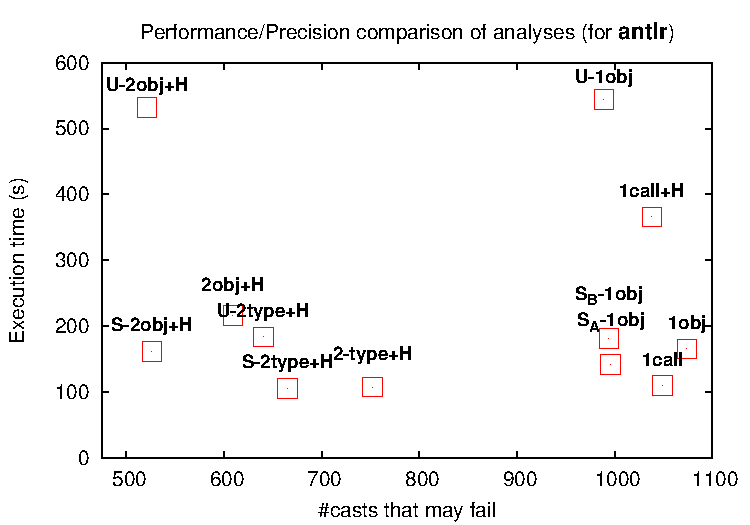
\includegraphics[width=\textwidth]{assets/hybrid/antlr.pdf}
\end{subfigure}\hspace{1cm}%
\begin{subfigure}[b]{0.45\textwidth}
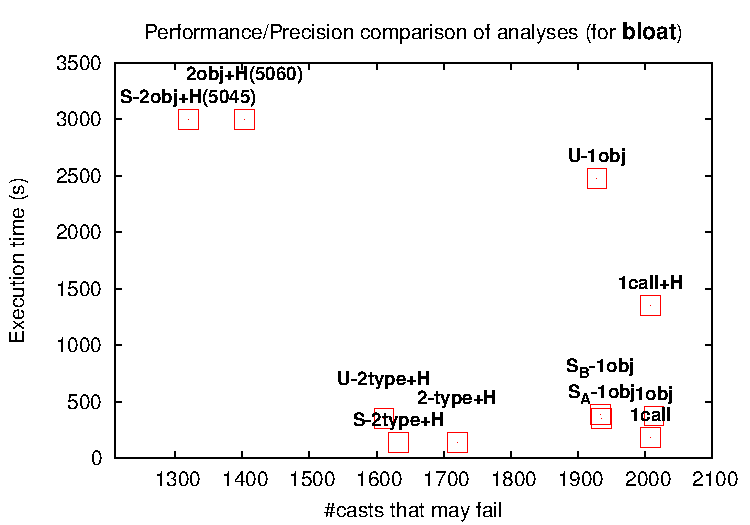
\includegraphics[width=\textwidth]{assets/hybrid/bloat.pdf}
\end{subfigure}
\begin{subfigure}[b]{0.45\textwidth}
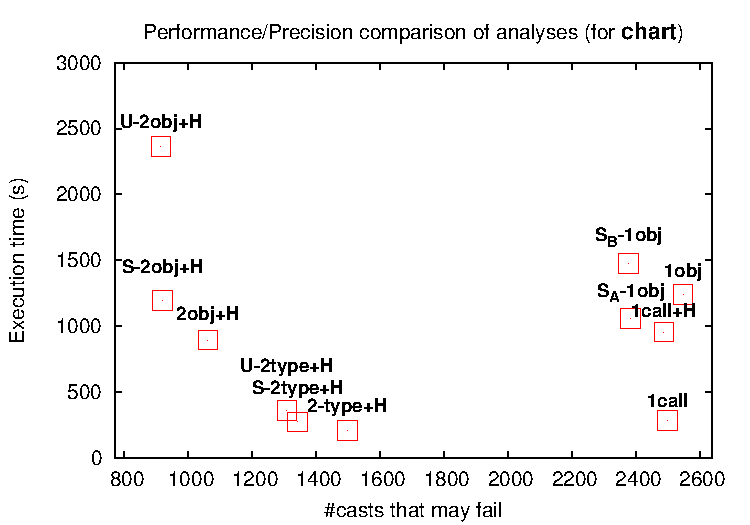
\includegraphics[width=\textwidth]{assets/hybrid/chart.pdf}
\end{subfigure}\hspace{1cm}%
\begin{subfigure}[b]{0.45\textwidth}
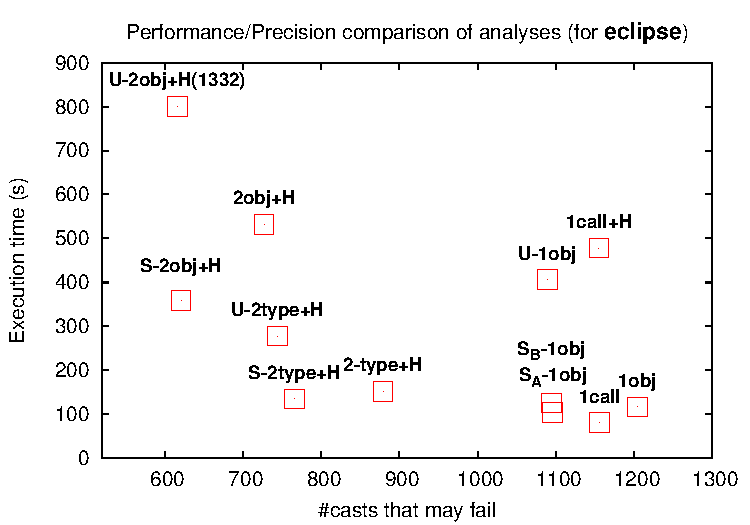
\includegraphics[width=\textwidth]{assets/hybrid/eclipse.pdf}
\end{subfigure}
\begin{subfigure}[b]{0.45\textwidth}
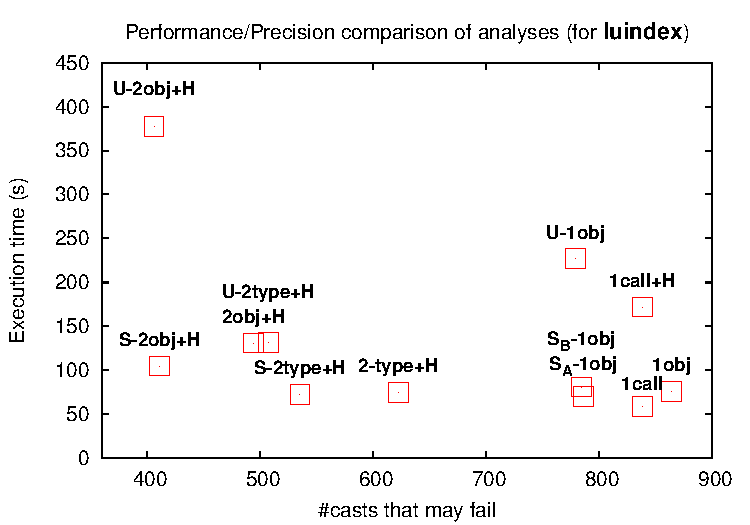
\includegraphics[width=\textwidth]{assets/hybrid/luindex.pdf}
\end{subfigure}\hspace{1cm}%
\begin{subfigure}[b]{0.45\textwidth}
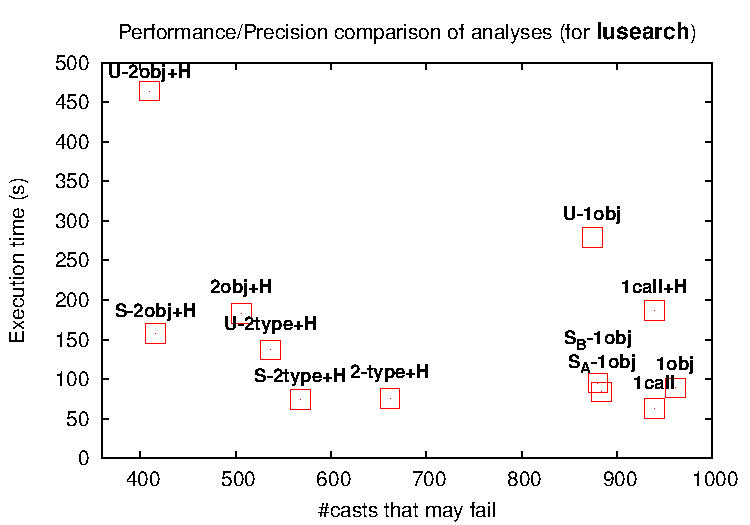
\includegraphics[width=\textwidth]{assets/hybrid/lusearch.pdf}
\end{subfigure}
\begin{subfigure}[b]{0.45\textwidth}
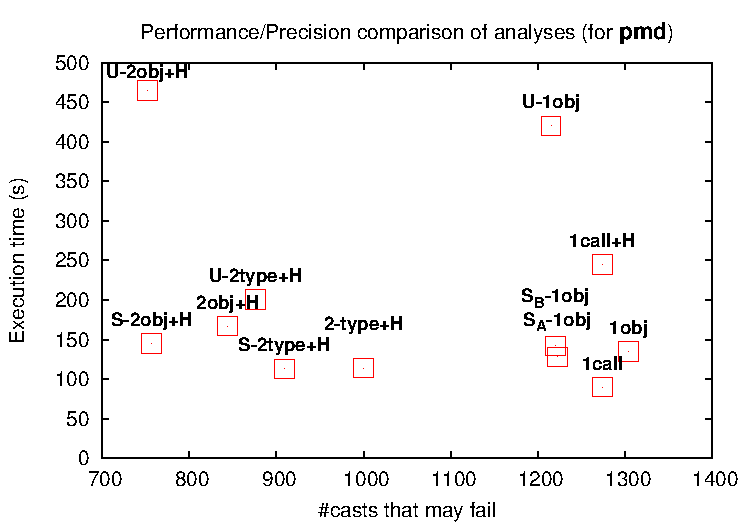
\includegraphics[width=\textwidth]{assets/hybrid/pmd.pdf}
\end{subfigure}\hspace{1cm}%
\begin{subfigure}[b]{0.45\textwidth}
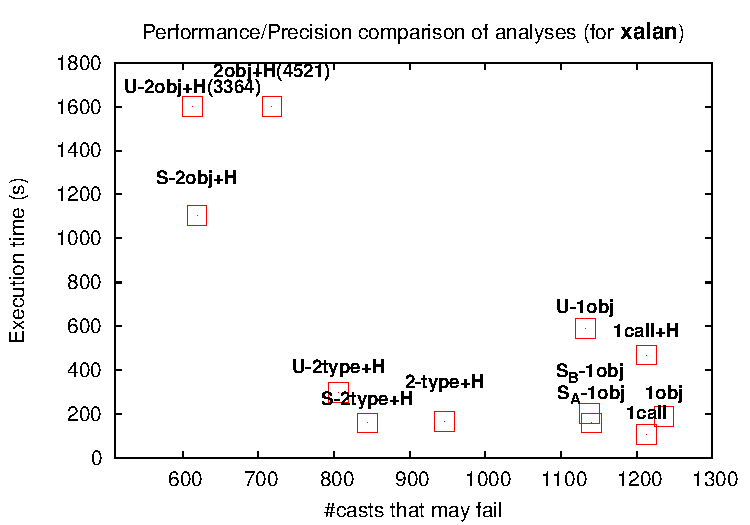
\includegraphics[width=\textwidth]{assets/hybrid/xalan.pdf}
\end{subfigure}
\caption{Graphical depiction of performance vs. precision metrics for
eight of our benchmarks over all analyses. Lower is better on both axes.
The Y axis is truncated for readability. Out-of-bounds points are included
at lower Y values, with their real running time in parentheses.
%The X axis (execution time) is truncated for readability, omitting
%1call+H and U-1obj for antlr and U-2obj+H for luindex.}
}
\label{fig:precision}
\end{center}
\end{figure*}

For an illustration of the precision and performance spectrum,
consider Figure~\ref{fig:precision}, which plots analyses on
precision/performance axes. The figure plots execution time against
precision in the ``may-fail casts'' metric, i.e., the number of casts
that the analysis cannot statically prove safe.  Lower numbers are
better on both axes, thus an analysis that is to the left and below
another is better in both precision and performance.  Values that are
disproportionately high on the Y axis (i.e., large execution times)
are clipped and plotted at the top of the figure, with the actual
number included in parentheses. (Note that the Y axis starts at zero,
while the X axis starts at an arbitrary point---we cannot know what is
the ``ideal'' reference value for this metric.)

In terms of pre-existing analyses, Figure~\ref{fig:precision}
illustrates what has been past experience: 2obj+H is the most precise
analysis, but often heavy. 1obj and 2type+H are both quite fast, with
2type+H also showing very good precision, often approaching
2obj+H. The two call-site-sensitive analyses (1call, 1call+H) are
mostly shown for reference and to demonstrate the insights discussed
in Section~\ref{sec:hybrid}. 1call is a fast analysis but vastly
imprecise, while 1call+H is a bad tradeoff: its cost grows quite
significantly relative to 1call without much precision
added---call-site sensitivity is a bad choice for heap contexts.

As can be seen, the selective hybrid analyses (S$_A$-1obj, S$_A$-1obj,
S-2obj+H, S-2type+H) usually offer an advantage over the
corresponding base analysis (1obj, 2type+H, 2obj+H) in both precision
and performance. In fact, selective hybrids are typically
imperceptibly less precise than the corresponding uniform hybrid, yet
much more precise than the base analysis. For instance, the plot
points for S-2obj+H are always barely to the right of those for the
theoretically more precise U-2obj+H (but significantly lower---uniform
hybrids are very expensive), while they are clearly to the left of
2obj+H.


\subsection{Detailed Results}

Detailed results of our experiments are presented in
Table~\ref{tab:results}.  The table shows precision and performance
metrics for all analyses. The precision metrics are the average
points-to set size (i.e., average over all variables of their
points-to sets sizes), the number of edges in the computed call-graph
(which is typically a good proxy for the overall precision of the
analysis, in broad strokes), and the results of two client analyses:
the number of virtual calls that could not be de-virtualized, and the
number of casts that could not be statically proven safe. A
combination of these four metrics gives a reliable picture of the
precision of an analysis. (Note that the average points-to set size
alone is not necessarily reliable, because it is influenced by a small
number of library variables with enormous points-to sets.  For
comparison, the \emph{median} points-to set size is 1, for all
analyses and benchmarks.)

\begin{table*}
\centering
\scalebox{0.9}{
\begin{tabular} {|c|r|r|r!{\vrule width 2pt}r|r|r|r!{\vrule width 2pt}r|r|r!{\vrule width 2pt}r|r|r|} %p{10cm}}
\cline{3-14}
\multicolumn{2}{c|}{} &
\multicolumn{1}{|c|}{\rotatebox{70}{\mbox{1call }}} &
\multicolumn{1}{|c!{\vrule width 2pt}}{\rotatebox{70}{\mbox{1call+H }}} &
\multicolumn{1}{|c|}{\rotatebox{70}{\mbox{1obj }}} &
\multicolumn{1}{|c|}{\rotatebox{70}{\mbox{U-1obj }}} &
\multicolumn{1}{|c|}{\rotatebox{70}{\mbox{S$_A$-1obj }}} &
\multicolumn{1}{|c!{\vrule width 2pt}}{\rotatebox{70}{\mbox{S$_B$-1obj }}} &
\multicolumn{1}{|c|}{\rotatebox{70}{\mbox{2obj+H }}} &
\multicolumn{1}{|c|}{\rotatebox{70}{\mbox{U-2obj+H }}} &
\multicolumn{1}{|c!{\vrule width 2pt}}{\rotatebox{70}{\mbox{S-2obj+H }}} &
\multicolumn{1}{|c|}{\rotatebox{70}{\mbox{2type+H }}} &
\multicolumn{1}{|c|}{\rotatebox{70}{\mbox{U-2type+H }}} &
\multicolumn{1}{|c|}{\rotatebox{70}{\mbox{S-2type+H }}} \\
\cline{1-14}
	
\multirow{6}{*}{\rotatebox{90}{\mbox{antlr}}}
& avg. objs per var          & 29.79 & 29.58 & 24.86 & 24.55 & 24.90 & 24.61 & 6.42 & 6.26 & 6.27 & 17.60 & 7.14 & 17.39 \\
& edges (over $\sim$8.8K meths) & 60999 & 60999 & 60194 & 60194 & 60202 & 60194 & 55548 & 55548 & 55548 & 55850 & 55765 & 55850 \\
& poly v-calls (of $\sim$33K)   & 1994 & 1994 & 1933 & 1933 & 1936 & 1933 & 1707 & 1707 & 1707 & 1759 & 1746 & 1759 \\
& may-fail casts (of $\sim$1.7K)     & 1049 & 1038 & 1074 & 989 & 996 & 994 & 609 & 521 & 526 & 752 & 640 & 665 \\
\cline{2-14}
& elapsed time (s)           & 110 & 366 & 166 & 544 & {\bf 142} & 182 & 217 & 532 & {\bf 162} & 108 & 184 & {\bf 106} \\
& sensitive var-points-to (M)    & 16 & 54.8 & 14.3 & 65 & {\bf 10.5} & 17.3 & 19.9 & 39.5 & {\bf 13.9} & 5.3 & 8.9 & {\bf 4.8} \\
\cline{1-14}

\multirow{6}{*}{\rotatebox{90}{\mbox{bloat}}}
& avg. objs per var          & 43.96 & 43.94 & 41.26 & 41.16 & 41.32 & 41.18 & 13.25 & - & 13.10 & 16.28 & 14.71 & 16.10 \\
& edges (over $\sim$10.2K meths) & 70506 & 70506 & 69501 & 69501 & 69511 & 69501 & 60726 & - & 60726 & 62115 & 61753 & 62115 \\
& poly v-calls (of $\sim$31K)   & 2138 & 2138 & 2076 & 2076 & 2080 & 2076 & 1640 & - & 1640 & 1888 & 1827 & 1888 \\
& may-fail casts (of $\sim$2.8K)     & 2008 & 2008 & 2013 & 1928 & 1935 & 1933 & 1403 & - & 1320 & 1720 & 1611 & 1633 \\
\cline{2-14}
& elapsed time (s)           & 186 & 1351 & 374 & 2473 & {\bf 353} & 391 & 5060 & - & {\bf 5045} & 142 & 353 & {\bf 140} \\
& sensitive var-points-to (M)    & 32.9 & 150.5 & 21.9 & 287.1 & {\bf 20.1} & 24 & 153.5 & - & {\bf 149.8} & 11.4 & 30.3 & {\bf 11} \\
\cline{1-14}

\multirow{6}{*}{\rotatebox{90}{\mbox{chart}}}
& avg. objs per var          & 45.12 & 45.11 & 40.80 & - & 40.72 & 40.11 & 5.30 & 4.99 & 5.00 & 7.02 & 5.89 & 6.57 \\
& edges (over $\sim$15K meths) & 82156 & 82078 & 81423 & - & 81075 & 81012 & 59162 & 59142 & 59152 & 62290 & 62172 & 62280 \\
& poly v-calls (of $\sim$35K)   & 2900 & 2897 & 2821 & - & 2815 & 2808 & 1610 & 1603 & 1610 & 1775 & 1756 & 1775 \\
& may-fail casts (of $\sim$3.5K)     & 2500 & 2488 & 2548 & - & 2385 & 2378 & 1062 & 915 & 920 & 1498 & 1309 & 1343 \\
\cline{2-14}
& elapsed time (s)           & 288 & 957 & 1240 & - & {\bf 1059} & 1477 & {\bf 896} & 2363 & 1199 & {\bf 211} & 362 & 276 \\
& sensitive var-points-to (M)    & 49.6 & 120.9 & 62.5 & - & {\bf 39.7} & 89.7 & 67.6 & 115.7 & {\bf 53} & {\bf 13.3} & 21.3 & 16.5 \\
\cline{1-14}

\multirow{6}{*}{\rotatebox{90}{\mbox{eclipse}}}
& avg. objs per var          & 21.84 & 21.65 & 18.65 & 18.41 & 18.59 & 18.43 & 5.75 & 5.60 & 5.61 & 7.93 & 6.41 & 7.61 \\
& edges (over $\sim$9.3K meths) & 53006 & 53001 & 52114 & 51935 & 51958 & 51936 & 44900 & 44899 & 44900 & 45318 & 45123 & 45235 \\
& poly v-calls (of $\sim$23K)   & 1515 & 1514 & 1429 & 1404 & 1412 & 1404 & 1163 & 1163 & 1163 & 1233 & 1202 & 1229 \\
& may-fail casts (of $\sim$2K)     & 1156 & 1155 & 1204 & 1089 & 1096 & 1094 & 727 & 616 & 621 & 879 & 744 & 766 \\
\cline{2-14}
& elapsed time (s)           & 81 & 478 & 117 & 406 & {\bf 105} & 126 & 532 & 1332 & {\bf 359} & 152 & 278 & {\bf 135} \\
& sensitive var-points-to (M)    & 12.3 & 61.5 & 9.4 & 42.3 & {\bf 7.6} & 10.8 & 44.6 & 89.8 & {\bf 32.3} & 13.6 & 24.4 & {\bf 11.5} \\
\cline{1-14}

\multirow{6}{*}{\rotatebox{90}{\mbox{hsqldb}}}
& avg. objs per var            & 18.56 & 18.53 & 15.41 & 15.30 & 15.58 & 15.32 & - &   -   & - & 7.92  & 6.71  & 7.74 \\
& edges (over $\sim$10K meths) & 54619 & 54619 & 53726 & 53724 & 53730 & 53724 & - &   -   & - & 49421 & 49319 & 49421 \\
& poly v-calls (of $\sim$26K)  &  1552 &  1552 & 1480  & 1479  &  1482 & 1479  & - &   -   & - & 1276  & 1263  & 1276 \\
& may-fail casts (of $\sim$2K) &  1360 &  1360 &  1385 &  1302 &  1320 &  1308 & - &   -   & - & 1031  & 923   & 948 \\
\cline{2-14}
& elapsed time (s)             &    90 &   332 &   218 &  1351 & {\bf 183} &   329 & - &   -   & - & {\bf 195}   & 583   & 238 \\
& sensitive var-points-to (M)  &  9.6    &    39.8 &    13.9 &    74.3 & {\bf   9.6} &    29.5 & - &   -   & - & {\bf  13.7} &    42.9 & 20.5 \\
\cline{1-14}

\multirow{6}{*}{\rotatebox{90}{\mbox{jython}}}
& avg. objs per var          & 20.64 & 20.57 & 18.21 & 18.01 & 18.19 & 18.09 & - & - & - & 8.55 & 7.18 & 8.30 \\
& edges (over $\sim$8.5K meths) & 50494 & 50480 & 49622 & 49614 & 49622 & 49614 & - & - & - & 43269 & 43138 & 43269 \\
& poly v-calls (of $\sim$21K)   & 1525 & 1524 & 1448 & 1448 & 1453 & 1448 & - & - & - & 1268 & 1236 & 1268 \\
& may-fail casts (of $\sim$1.9K)     & 1140 & 1140 & 1157 & 1087 & 1094 & 1092 & - & - & - & 909 & 822 & 840 \\
\cline{2-14}
& elapsed time (s)           & 88 & 401 & 119 & 375 & {\bf 102} & 138 & - & - & - & 731 & 1363 & {\bf 676} \\
& sensitive var-points-to (M)    & 10.4 & 50.6 & 8.7 & 43.2 & {\bf 6.7} & 10.8 & - & - & - & {\bf 52} & 118.4 & 56.5 \\
\cline{1-14}

\multirow{6}{*}{\rotatebox{90}{\mbox{luindex}}}
& avg. objs per var          & 17.65 & 17.58 & 14.94 & 14.81 & 14.97 & 14.83 & 4.77 & 4.55 & 4.55 & 6.20 & 5.15 & 5.92 \\
& edges (over $\sim$7.9K meths) & 41992 & 41992 & 41103 & 41103 & 41111 & 41103 & 36580 & 36580 & 36580 & 36889 & 36796 & 36889 \\
& poly v-calls (of $\sim$18K)   & 1180 & 1180 & 1119 & 1119 & 1122 & 1119 & 894 & 894 & 894 & 949 & 932 & 949 \\
& may-fail casts (of $\sim$1.4K)     & 838 & 838 & 864 & 779 & 786 & 784 & 494 & 406 & 411 & 622 & 507 & 535 \\
\cline{2-14}
& elapsed time (s)           & 59 & 172 & 76 & 227 & {\bf 70} & 81 & 131 & 377 & {\bf 105} & 75 & 132 & {\bf 73} \\
& sensitive var-points-to (M)    & 7.8 & 26.1 & 5.4 & 26.3 & {\bf 4.1} & 6.4 & 11.1 & 22.4 & {\bf 7.2} & 4.5 & 7.6 & {\bf 3.5} \\
\cline{1-14}

\multirow{6}{*}{\rotatebox{90}{\mbox{lusearch}}}
& avg. objs per var          & 18.64 & 18.47 & 15.71 & 15.57 & 15.79 & 15.60 & 4.71 & 4.49 & 4.50 & 6.13 & 5.10 & 5.86 \\
& edges (over $\sim$8.4K meths) & 45270 & 45270 & 44371 & 44365 & 44379 & 44371 & 39452 & 39446 & 39452 & 39763 & 39662 & 39763 \\
& poly v-calls (of $\sim$19K)   & 1360 & 1360 & 1299 & 1299 & 1302 & 1299 & 1065 & 1065 & 1065 & 1122 & 1103 & 1122 \\
& may-fail casts (of $\sim$1.5K)     & 939 & 939 & 961 & 874 & 884 & 880 & 506 & 410 & 416 & 662 & 537 & 568 \\
\cline{2-14}
& elapsed time (s)           & 63 & 187 & 89 & 279 & {\bf 84} & 95 & 183 & 464 & {\bf 158} & 76 & 137 & {\bf 74} \\
& sensitive var-points-to (M)    & 8.7 & 28.5 & 6.2 & 30.3 & {\bf 5.3} & 7.2 & 13.2 & 26.3 & {\bf 10} & 4.2 & 7.8 & {\bf 3.6} \\
\cline{1-14}

\multirow{6}{*}{\rotatebox{90}{\mbox{pmd}}}
& avg. objs per var          & 19.94 & 19.82 & 17.36 & 17.22 & 17.37 & 17.24 & 4.87 & 4.68 & 4.68 & 6.35 & 5.28 & 6.10 \\
& edges (over $\sim$9.2K meths) & 49097 & 49097 & 48250 & 48250 & 48258 & 48250 & 43068 & 43067 & 43067 & 43401 & 43315 & 43400 \\
& poly v-calls (of $\sim$21K)   & 1249 & 1249 & 1187 & 1187 & 1190 & 1187 & 937 & 937 & 937 & 988 & 976 & 988 \\
& may-fail casts (of $\sim$2K)     & 1274 & 1274 & 1304 & 1215 & 1222 & 1220 & 844 & 752 & 757 & 1000 & 876 & 909 \\
\cline{2-14}
& elapsed time (s)           & 90 & 245 & 135 & 420 & {\bf 128} & 142 & 167 & 465 & {\bf 145} & 114 & 201 & {\bf 113} \\
& sensitive var-points-to (M)    & 11.4 & 35.9 & 7.9 & 42.6 & {\bf 6.9} & 9.2 & 13.2 & 30.5 & {\bf 10} & 4.5 & 9.7 & {\bf 3.9} \\
\cline{1-14}

\multirow{6}{*}{\rotatebox{90}{\mbox{xalan}}}
& avg. objs per var          & 25.50 & 25.38 & 21.86 & 21.59 & 21.84 & 21.69 & 5.48 & 5.22 & 5.23 & 7.52 & 6.19 & 7.16 \\
& edges (over $\sim$10.5K meths) & 57168 & 57168 & 56412 & 56158 & 56404 & 56395 & 50148 & 50054 & 50054 & 50539 & 50432 & 50526 \\
& poly v-calls (of $\sim$26K)   & 1976 & 1976 & 1920 & 1905 & 1921 & 1918 & 1619 & 1615 & 1615 & 1677 & 1660 & 1677 \\
& may-fail casts (of $\sim$2K)     & 1213 & 1213 & 1236 & 1132 & 1140 & 1138 & 718 & 613 & 619 & 946 & 806 & 844 \\
\cline{2-14}
& elapsed time (s)           & 108 & 470 & 189 & 591 & {\bf 161} & 205 & 4521 & 3364 & {\bf 1105} & 168 & 299 & {\bf 161} \\
& sensitive var-points-to (M)    & 14.5 & 59.8 & 15.5 & 67.5 & {\bf 10.9} & 18.2 & 166.6 & 171.7 & {\bf 63.3} & 10.2 & 17.4 & {\bf 9} \\
\cline{1-14}

\end{tabular}
}
\caption[]{Precision and performance metrics for all benchmarks and
analyses, grouped by relevance. In all cases \emph{lower is
better}. Dash (-) entries are for analyses that did not terminate in
90mins.  The 4 precision metrics shown are the average size of
points-to sets (how many heap objects are computed to be pointed-to
per-var), the number of edges in the computed call-graph, the number
of virtual calls whose target cannot be disambiguated by the analysis,
and the number of casts that cannot be statically shown safe by the
analysis. Reference numbers (e.g., total reachable casts in the
program) are shown in parentheses in the metric's heading.  These
numbers change little per-analysis. Performance is shown as running
time and size of context-sensitive var-points-to data (the main
platform-independent internal complexity metric). Best performance
numbers per-analysis-group are \textbf{in bold}.}
\label{tab:results}
\end{table*}


Performance is shown with two metrics: time and total size of all
\emph{context-sensitive} points-to sets. Although time is the ultimate
performance metric, it is brittle: one can argue that our time
measurements are influenced by a multitude of implementation or
environment factors, among which are the choice of underlying data
structures, indexing, and the overall implementation of the points-to
analysis, especially since it is running on a Datalog engine, with its
own complex implementation choices hidden. The context-sensitive
points-to set size metric does not suffer from any such measurement or
implementation bias. It is the foremost internal complexity metric of
a points-to analysis, and typically correlates well with time, for
analyses of the same flavor.  Note that analysis implementations that
fundamentally differ from ours also try hard to minimize this metric
in order to achieve peak performance: Lhot\'{a}k's \textsc{Paddle}
framework \cite{thesis:Lhotak} is using binary decision diagrams
(BDDs) for representing relations. The best BDD variable ordering
(yielding ``impressive results'' \cite{pldi:2003:Berndl})
is one that minimizes the total size of context-sensitive points-to
sets. In short, it is reasonable to expect that improvements in this
internal metric reinforce the verdict of which analysis yields better
performance, not just in our setting but generally. Furthermore, the
size of context-sensitive points-to sets serves as a valuable
indicator of the internally different computation performed by various
analyses: Analyses with almost identical precision metrics (e.g.,
context-insensitive points-to set sizes, call-graph edges) have vastly
different context-sensitive points-to set sizes.


Since Table~\ref{tab:results} has a high information density, we guide
the reader through some of the most important findings below (see also
a partial illustration in Figure~\ref{fig:precision}, later).

\begin{itemize}

\item \textbf{\emph{General observations.}}
The analyses shown are in 4 
groups of closely related analyses: call-site sensitive,
1-object-sensitive, 2-object-sensitive with a 1-context-sensitive
heap, and 2-type-sensitive with a 1-context-sensitive heap. 
These analyses span a large performance and precision spectrum.
For instance, for the chart benchmark, the least precise analysis,
1call, runs for under 5mins and computes an average points-to size of
over 45, while the most precise, U-2obj+H, runs for over 53mins and
computes an average points-to size of under 5. The difference in
precision is also vividly shown in the ``may-fail casts'' metric: the
1call analysis cannot prove 2500 casts safe, while the U-2obj+H fails
to prove safe just 915 casts (both numbers from a total of about 3.5K
reachable casts---the exact number varies slightly due to method
reachability variation per analysis). 

% Specifically, 1call, 1obj, and 2type+H are
%the fastest analyses in our set (for different programs each), with
%each one offering significant precision enhancements relative to the
%previous. 2obj+H is typically slower but manageable, and achieves
%very high precision.

\item \textbf{\emph{Uniform hybrid analyses.}}  Recall that uniform
hybrid analyses (U-1obj, U-2obj+H, U-2type+H) were defined to always
keep a combination of object-sensitive and call-site-sensitive
context. As a result, the analyses are more precise than their
respective base analyses (1obj, 2obj+H, 2type+H), especially in the
``may-fail casts'' metric. However, this precision comes at great
cost: uniform hybrid analyses are often 3x or more slower than their
base analyses with twice as large, or more, context-sensitive
points-to sets. U-1obj and U-2obj+H are plainly bad tradeoffs in the
design space: for a slight increase in precision, the performance cost
is heavy. U-2type+H is a bit more reasonable: it achieves more
significant precision gains and its performance toll is often under 2x
while still terminating comfortably for all our benchmarks. In fact, a
surprising finding was that U-2type+H is a tempting alternative to
2obj+H for applications that need very high precision, given its good
scalability.
%It is most likely
%due to the specific nature of type-sensitive analyses: the class in
%which a receiver object is allocated forms a good differentiator of
%behavior when combined with a call-site.

\item \textbf{\emph{1obj hybrids.}}
We presented two selective hybrids of a 1-object-sensitive analysis:
S$_A$-1obj (which keeps either an allocation site or a call-site as
context, but not both) and S$_B$-1obj (which always keeps an
allocation site as context and occasionally adds a call-site to
it). They both turn out to be interesting analyses from a practical
standpoint. The former is consistently faster than the base 1obj
analysis, with roughly similar precision and occasionally (for the
``may-fail casts'' metric) higher precision. The size of
context-sensitive points-to sets also confirms that this is a
``lighter'' analysis that is likely to cost less in any context. The
S$_B$-1obj analysis is always more precise than 1obj (as is statically
guaranteed) for a slight extra cost. Indeed, S$_B$-1obj is a good
approximation of the uniform hybrid analysis, U-1obj, in terms of
precision, for a fraction (typically less than a third) of the cost.

\item \textbf{\emph{2obj+H hybrids.}}  The selective hybrid idea
yields even more dividends when applied to the very precise 2obj+H
analysis. S-2obj+H is more precise than 2obj+H and only very slightly
less precise than the uniform hybrid, U-2obj+H. In terms of
performance, however, the analysis is typically well over 3 times
faster than U-2obj+H, and significantly faster (an average of 53\%
speedup) than 2obj+H. This is interesting, given the practical value
of 2obj+H, since it establishes a new sweet spot in the space of
relatively scalable but highly precise analyses: S-2obj+H is both more
precise than 2obj+H (especially for ``may-fail casts'') and
substantially faster.

\item \textbf{\emph{2type+H hybrids.}} The 2type+H analysis variations
are also highly interesting in practice. This is an analysis space
that yields excellent precision relative to its low cost. There are
few cases in which one might prefer some other inexpensive analysis
over 2type+H given the combination of precision and competitive
performance of the latter. As we saw, the uniform hybrid, U-2type+H,
is an interesting tradeoff in this space. The selective hybrid,
S-2type+H, also performs quite well. It is just as fast or slightly
faster than the base analysis 2type+H, while also being more precise.

\end{itemize}


\section{Related Work}
\label{sec:related}

We have discussed directly related work throughout the paper. Here we
selectively mention a few techniques that, although not directly
related to ours, offer alternative approaches to sweet spots in the
precision/performance tradeoff.

Special-purpose combinations of context-sensitivity have been used in
the past, but have required manual identification of classes to be
treated separately (e.g., Java collection classes, or library factory
methods). An excellent representative is the TAJ work for taint
analysis of Java web applications
\cite{pldi:2009:Tripp}. In contrast, we have sought to
map the space and identify interesting hybrids for general application
of context-sensitivity, over the entire program.

The analyses we examined are context-sensitive but flow-insensitive.
We can achieve several of the benefits of flow-sensitivity by applying
the analysis on the static single assignment (SSA) intermediate form
of the program. This is easy to do with a mere flag setting on the
\doop{} framework. However, the impact of the SSA transformation
on the input is minimal. The default intermediate language used as
input in \doop{} (the Jimple representation of the Soot
framework \cite{cascon:1999:Vall,cc:2000:Vall}) is already close to
SSA form, although it does not guarantee that every variable is
strictly single-assignment without requesting it explicitly.  Recent
work by Lhot\'{a}k and Chung \cite{popl:2011:Lhotak} has shown that
much of the benefit of flow-sensitivity derives from the ability to do
strong updates of the points-to information. Lhot\'{a}k and Chung then
exploited this insight to derive analyses with similar benefit to a
full flow-sensitive analysis at lower cost.

A demand-driven evaluation strategy reduces the cost of an analysis by
computing only those results that are necessary for a client program
analysis~\cite{oopsla:2005:Sridharan,pldi:2006:Sridharan,popl:2008:Zheng,pldi:2001:Heintze}. This is a useful
approach for client analyses that focus on specific locations in a
program, but if the client needs results from the entire program, then
demand-driven analysis is typically slower than an exhaustive
analysis.

Reps~\cite{cc:1994:Reps} showed how to use the standard magic-sets
optimization to automatically derive a demand-driven analysis
from an exhaustive analysis (like ours). This optimization
combines the benefits of top-down and bottom-up evaluation of
logic programs by adding side-conditions to rules that limit
the computation to just the required data.

An interesting recent approach to demand-driven analyses was
introduced by Liang and Naik \cite{pldi:2011:Liang}.
Their ``pruning'' approach consists of first computing a coarse
over-approximation of the points-to information, while keeping the
provenance of this derivation, i.e., recording which input facts have
affected each part of the output. The input program is then pruned so
that parts that did not affect the interesting points of the output
are eliminated. Then a precise analysis is run, in order to establish
the desired property.

\section{Conclusions and Future Work}

We presented a comprehensive map for the exploration of context
combinations in points-to analysis, and used it to discover several
interesting design points. Object-sensitivity and
call-site-sensitivity had never been fruitfully combined in the past,
although the idea is clearly tempting. We speculate that the reasons
for the paucity of hybrid context-sensitivity results have been a) the
difficulty of having a good enough model for the space of combinations
and a convenient implementation to explore it; b) a belief that
nothing fruitful will come out of such a combination, because
call-site sensitivity incurs a high performance cost, which is more
profitably spent on an extra level of object-sensitivity. The latter
insight is mostly true, but only if one considers uniform hybrid
analyses. As we saw, much of the benefit of call-site and
object-sensitive hybrids comes from allowing the context to vary
between pure object-sensitive and extended. The result of our work has
been new sweet spots, in both precision and performance, for some of
the most practically relevant analysis variations.

There are several interesting directions for further work that open
up. First, our model gives the ability for further experimentation,
e.g., with deeper-context analyses. Furthermore, it is interesting to
examine if a hybrid context should perhaps change form more
aggressively. The \consname{Merge} and \consname{MergeStatic}
functions could examine the context passed to them as argument and
create different kinds of contexts in return. For instance, the
context of a statically called method could have a different form
(e.g., more elements) for a call made inside another statically called
method vs. a call made in a virtual method. Similarly, objects could
have different context, via the \consname{Record} function, depending
on the context form of their allocating method. To explore this space
without blind guessing, one needs to understand what programming
patterns are best handled by hybrid contexts and how. For deep
contexts this remains a challenge, as it is hard to reason about how
context elements affect precision. (E.g., past work had to offer
involved arguments for why the allocator object of the receiver object
of a method is a better context element than the caller object 
\cite{popl:2011:Smaragdakis}.) This challenge is, however, worth addressing
for the next level of benefit in context-sensitive points-to analysis.
